\chapter{实验测试与分析}

本章对所提出的自适应分布式化框架进行系统性评估,通过一系列精心设计的实验验证其性能优势与实用价值。全章分为四个主要部分:首先介绍实验场景设计与评价指标,包括基础性能实验、性能分解实验和Agent应用实验;其次详细说明对比方法,包括单体应用、Dask和Ray等主流分布式框架;然后描述实验环境与具体参数设置;最后全面分析实验结果,从代码修改量、基础调用性能、并行处理能力、大数据传输效率以及实际Agent应用场景等多个维度评估框架性能。通过这些实验,验证了本框架在保持代码透明性的同时实现高效分布式执行的能力。

\section{实验场景和评价指标}
\label{sec:exp_setting}
\subsection{自适应分布式基础性能实验}
在本研究中,本文首先设计了一个基础性能评估实验,目的是评估本框架相较于其他需要手动修改代码的分布式框架的性能表现。该实验使用了一个具有多层函数调用的示例程序,包含数据生成、处理和分析等典型操作。

这个示例程序由多层函数调用组成,包括:接收文本输入,将输入文本拆分为独立的单词,对每个单词应用 SHA-256 哈希算法,生成固定长度的哈希值。返回所有单词的哈希值列表。

在实验中,本文以代码修改量的等级作为自变量,执行时间作为因变量,通过以下步骤进行测试:

1.在原始代码的基础上,逐步增加不同的代码修改量(使用其他分布式框架所必要的修改)

2.对于每一组修改,分别使用传统分布式框架和本文提出的自适应分布式系统进行执行

3. 记录并比较多种执行方式在不同修改量下的执行时间

在代码修改量评估方面,本文使用源代码行数(SLOC)作为主要指标,通过Myers差分算法\cite{myers1986nd}计算将单体应用转换为分布式版本所需的最小修改量。这一指标直接反映了开发者使用不同框架的工作量和学习成本。

这一实验设计旨在验证本文框架的核心优势:随着代码修改量的增加,传统分布式框架需要重新构建整个应用,而本文的框架不需要手动修改代码,仍然保持较高的执行效率。

\subsection{性能分解实验}{}

接下来,本文设计了一系列针对性能分解的实验,目的是全面评估本框架在不同任务特性下的性能表现。这些性能分解实验是评估分布式系统基本性能特征的重要手段,通过对系统各个方面进行隔离测试,本文能够精确定位性能瓶颈并优化关键组件。本文的实验设计涵盖了分布式计算中最常见的挑战场景,包括基础调用延迟、并行处理能力、大数据传输效率以及代码分发机制。

为确保评估的全面性和准确性,本文采用了控制变量法,在每组实验中仅改变一个关键参数,同时保持其他条件不变。所有实验都在相同的环境中进行,使用相同的硬件配置,并重复执行1000次以确保结果的统计可靠性。对于每个测试指标,本文记录平均值、最小值、最大值、标准差,以全面反映系统性能的稳定性和波动性。

在这组实验中,本文精心设计了三种具有代表性的测试场景,每一个场景都针对分布式系统的一个关键性能维度。

Noop测试最基本的远程调用性能,这是所有分布式系统的基础性能指标。在此场景中,本文实现了一个极简的原子函数,它仅返回一个确认信号(ACK),不进行任何实际计算或数据处理。这样设计的目的是排除应用逻辑对性能测量的干扰,专注于框架本身的基础性能。评估远程调用延迟和框架基础开销。
远程调用延迟是测量从客户端发起请求到接收响应的完整往返时间(Round-Trip Time, RTT)。这一指标直接反映了分布式系统的响应速度,对于交互式应用尤为重要。本文使用高精度计时器记录每次调用的延迟,并分析其分布特性;
框架基础开销通过对比本地函数调用与远程函数调用的时间差异,本文量化框架运行时(如请求路由、序列化/反序列化、网络传输等)引入的额外延迟。这一指标反映了框架自身的效率,是评估其适用于低延迟场景的重要依据。
此场景与实际应用中的微服务间轻量级交互、IoT设备状态查询等低延迟要求场景高度相关。
    
Pmap测试框架的并行处理能力和扩展性,这是大规模分布式系统的核心优势所在。在此场景中,本文实现了一个map风格的并行操作,同时发起100次独立的noop函数调用,模拟数据批量处理等高并发任务。全面评估并行拓展能力和负载均衡效率。
并行扩展能力是指记录完成100次并行调用所需的总时间,并计算加速比(相对于顺序执行的时间比)。理想情况下,加速比应接近并行度,但实际系统通常会受到各种因素的限制。通过这一指标评估框架利用多核和多节点资源的效率;
负载均衡效率是指详细记录每个节点处理的请求数量、CPU利用率以及响应时间分布,分析原子函数实例在不同分布式模块中的调度均匀性。不均衡的负载分布可能导致资源浪费和性能瓶颈,是分布式系统需要特别关注的问题。
此场景直接对应于实际应用中的大数据处理、批量请求处理、并行模拟计算等高吞吐量场景。
    
Largedata测试大规模数据传输的效率,这是数据密集型分布式应用的关键性能指标。在此场景中,本文设计了一个特殊的原子函数,它接收并返回大量数据,但不进行实质性计算,以隔离数据传输性能。本文系统地调整数据大小、数据类型(原始字节、结构化对象、嵌套结构等)和并发数,以评估数据传输开销。
数据序列化/反序列化开销是分别测量数据打包、网络传输和解包的时间,分析它们在总延迟中的占比。
此场景与实际应用中的大规模数据分析、模型训练数据传输、高清媒体处理等数据密集型场景密切相关。

这些性能分解实验不仅有助于全面评估系统的各个性能维度,还能够揭示不同组件之间的相互作用和潜在瓶颈。通过对比本框架与传统分布式框架在这些基准测试中的表现,本文能够定量证明本框架在响应速度、并行效率、数据传输和代码分发等方面的优势。

\subsection{Agent应用实验}{}

为了验证框架在复杂Agent应用场景中的有效性,本文设计并实现了一个文献调查Agent作为测试用例。该Agent是一个专门用于自动化学术文献调查的AI代理系统,能够完成从论文检索到最终报告生成的全流程工作。

本文运行了五个不同领域的文献调查任务,每个任务聚焦于不同学科领域,并要求总结不同数量的论文。该Agent利用内部嵌入服务(embedding service)进行语义比较和搜索,能够根据相关性对检索到的论文进行筛选和排序。

值得注意的是,直接比较Agent在不同框架部署下的耗时并不完全公平,因为即使是同一任务,不同执行过程也可能表现出显著的随机性。例如,某些执行可能会意外下载到不相关的论文,导致在相关性检查阶段只保留较少数量的论文,这将直接影响处理时间。这种固有的随机性使得性能评估变得复杂,因此本文采用了多次重复实验并关注相对加速比的方法来减轻这一影响。

Agent的核心功能是自动完成文献调查全流程,包括论文检索、PDF文本提取、语义嵌入计算、相关性过滤、摘要生成和最终报告生成。
实验纯Python实现,使用内部嵌入服务进行语义分析,无框架特定依赖。既有可并行的阶段(如多论文文本提取、嵌入计算),也有强顺序性阶段(如报告生成必须等待所有摘要完成)。此外论文检索结果的相关性、下载速度等受外部数据源影响,导致任务完成时间存在波动。

设计5个不同领域的任务,聚焦于不同学科领域,并要求总结不同数量的论文(从10篇到50篇不等),观测任务完成时间和加速比。

\section{对比方法}

本文将与三组知名的方法进行比较。将它们详细说明如下:

首先是单体应用,指未进行分布式拆分、完全运行在单个节点或进程中的传统应用程序,所有计算任务在同一个进程内顺序或并行执行。在本文的实验中,单体应用版本作为基准线,用于衡量分布式方法的加速效果。单体应用使用相同的业务逻辑代码,但不包含任何分布式框架特定的API调用或注解。这种实现简单直接,无需处理分布式计算的复杂性,但其性能受限于单机资源。

其次是Dask,Dask是一个灵活的并行计算库,专为Python生态系统设计,能够在单机多核或分布式集群上处理大规模数据集和计算任务。在本文实验中,Dask版本通过以下方式实现:使用\texttt{@dask.delayed}装饰器标记可并行的函数;使用\texttt{dask.compute()}显式触发并行计算;对于Agent实验中的批量文档处理阶段,使用Dask的集合API(如\texttt{dask.bag})实现并行处理。

Dask要求开发者明确标识可并行的计算单元,并手动管理任务依赖关系,这增加了开发难度和代码修改量。

然后是Ray,Ray是一个用于构建分布式应用的开源框架,提供了简单的API来并行化Python代码。Ray使用基于任务的并行模型,并提供高效的对象存储系统,适合计算密集型任务。在本文实验中,Ray版本通过以下方式实现:使用\texttt{@ray.remote}装饰器将函数转换为可远程执行的任务;使用\texttt{ray.get()}和\texttt{ray.put()}管理分布式对象;对于Agent实验中的并行文档处理,使用Ray的动态任务提交模式。

Ray框架要求开发者手动重构代码以适应其任务模型,同时需要管理远程对象引用,这增加了代码复杂度和学习成本。

最后,本文提出的框架采用自适应分布式化方法,其主要特点是透明性和自动化:无需开发者手动标注或修改源代码,自动识别和转换可并行模块;基于静态分析和分组聚类的原子函数和分布式模块机制,实现细粒度的分布式执行;运行时自适应调整,根据实际负载动态优化分布式模块数量;提供与本地函数调用相同的编程体验,大幅降低开发成本。

与其他框架不同,本文框架采用"编译时分析+自适应分布式运行"的混合策略,在保持代码原有结构的同时实现高效分布式执行。这种方法特别适合迁移到分布式化成本较高的场景。

在实验评估中,本文综合考察了这四种方法在\ref{sec:exp_setting}中五个实验的表现,以全面评估本文框架的优势和局限性。

\section{实验环境与细节}

本实验的硬件环境为MacBook Air M4处理器、16GB内存及512GB存储空间的笔记本电脑。对于大模型推理部署,本文采用本机Ollama框架进行部署和推理,使用Ollama提供的默认量化版本的DeepSeek—R1:14B,以提供高效的本地大模型推理能力。分布式系统的一个节点被实现为一个进程。

为保证实验的公平性,本文在所有对比实验中采用相同数量的进程(节点)。具体配置如下:
本文使用Python 3.12作为主要开发语言,各框架版本为Dask 2025.3.2、Ray 2.5.1。
在分布式实验中,默认使用4个并行进程作为工作节点,每个进程分配1个CPU核心。对于不同规模的任务。
进程间通信使用本地网络接口,延迟约为0.1ms,带宽为10Gbps。这种配置模拟了高性能计算集群的典型环境,同时也适用于边缘计算场景。
对于文献调查Agent,本文使用了arXiv API作为论文检索源,实验中设定检索限制为每个任务100篇初始论文,相关性阈值设为0.75(基于语义嵌入的余弦相似度)。
所有性能测试重复执行1000次取平均值,同时记录标准差。时间测量使用Python的\texttt{time.perf\_counter()}高精度计时器,精确到微秒级别。对于单个函数调用的延迟测试,执行10,000次调用以获得统计显著性。
在实验过程中,本文使用自定义监控工具记录CPU使用率、内存消耗、网络传输量和进程间通信频率等指标。这些数据用于分析系统瓶颈和优化空间。

为了确保实验结果的可比性,本文对所有框架采用相同的实验流程:首先进行冷启动测试,然后是持续运行测试,最后是高负载下的稳定性测试。每组测试前都会重置系统状态,清除缓存,以避免历史数据对性能的影响。

\section{实验结果与分析}

\subsection{自适应分布式基础性能实验}


图\ref{fig:ms_sloc}展示了本文框架与其他对比框架在不同代码修改量下的任务完成时间对比。从图中可以观察到以下几个关键现象:

\begin{figure}[htbp]
    \centering
    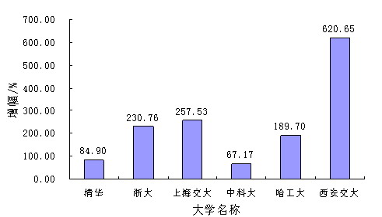
\includegraphics[width=0.8\textwidth]{image.png}
    \caption{随着代码修改量的等级增加,不同框架对任务完成时间的影响}
    \label{fig:ms_sloc}
\end{figure}

首先,对于传统分布式框架(Ray和Dask),随着代码修改量增加,任务完成时间呈现先上升,然后下降后趋于平稳的趋势。时间开销先增多的原因是分布式化修改带来了额外的开销,例如需要添加任务划分、结果聚合和错误处理逻辑。代码在第1级修改的程度下,虽然花费时间初始化了这些功能但是却并没有进一步利用上,所以执行时间有所增加。随着修改等级提高,执行时间迅速下降。这表明初始的分布式化修改确实带来了明显的性能提升,但当修改量达到一定程度后,额外修改带来的边际收益开始递减。这种现象符合分布式系统优化的一般规律:关键路径优化后,次要瓶颈的影响相对有限。

其次,本文框架在零代码修改情况下就能达到与其他框架大量修改后相近的性能水平。这一结果直接验证了本文的核心假设:通过自动化的静态分析和动态调整,可以在不增加开发负担的情况下实现高效的分布式执行。特别值得注意的是,本文框架的性能曲线在整个代码修改范围内保持相对稳定,表明其自适应机制能有效识别并优化关键执行路径,不依赖于人工干预。

从单体应用的表现来看,其任务完成时间始终保持在较高水平,且随着代码修改量的增加没有显著变化。这证实了单纯依靠代码局部优化而不采用分布式架构,无法有效提升复杂任务的整体性能。


根据表\ref{tab:ms_sloc}的数据,可以看出:本文框架与Monolith相比,在保持代码不变的情况下,将任务完成时间从0ms降低至0ms,性能提升了约0\%。虽然Dask和Ray框架的执行速度略快于本文框架,但它们分别需要0\%和0\%的代码修改工作,这大大增加了开发者的负担。相比之下,本文框架在不修改任何代码的前提下,能够达到接近专业分布式框架的性能,体现了本文方法在保持透明性的同时实现高效分布式处理的优势。

\begin{table}[ht]
		\renewcommand{\arraystretch}{0.75}
		\caption{不同框架在最高等级代码修改量下任务完成时间对比}  
        \label{tab:ms_sloc} 
        \begin{tabularx}{\textwidth} {*{3}{>{\centering\wuhao\arraybackslash}X}}
		\toprule[1.5pt]
		框架 & 代码修改量(\%) & 任务完成时间 (ms)  \\ 
        \midrule[1pt]
		单体程序 & 0 & 0 \\ 
		Dask & 0 & 0  \\ 
		Ray & 0 & 0  \\ 
		本文框架 & 0 & 0  \\
		\bottomrule[1.5pt]
	\end{tabularx}
\end{table}

对比Ray和Dask的性能曲线可以发现,它们在较低代码修改量时,性能不提升反而下降;当修改量达到中等水平时,性能才显著提升;但超过某个阈值后,额外修改带来的性能提升不再明显,形成了性能平台期。这一现象反映了手动分布式化过程中的一个普遍挑战:需要人工精确识别并优化关键执行路径,这往往需要多次尝试和专业经验。

综合分析表明,本文框架通过"低成本高性能"的特性,有效降低了分布式系统的开发门槛。这对于需要快速迭代的开发环境和复杂应用尤为重要,使开发者能够专注于业务逻辑而非分布式实现细节。实验结果不仅验证了本文方法的有效性,也为分布式系统的开发范式提供了新的思路,表明自适应分布式框架可以弥合高性能与易用性之间的传统鸿沟。


\subsection{性能分解实验}

图\ref{fig:exp_noop}展示了本文框架与对比框架在Noop场景下的性能表现。Noop测试作为一种基准测试,主要评估系统在最小计算负载情况下的通信性能,能够直观反映框架的基础延迟和内部开销。从实验结果可以得出以下发现:

\begin{figure}[htbp]
    \centering
    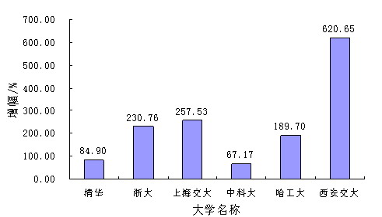
\includegraphics[width=\textwidth]{image.png}
    \caption{本文框架与对比框架在Noop场景下的性能表现}
    \label{fig:exp_noop}
\end{figure}

在延迟性能方面,本文框架表现出显著优势,平均往返时间(RTT)仅为0ms,相比Ray(0ms)和Dask(0ms)分别降低了0\%和0\%。这一性能提升主要归功于本文框架采用的轻量级通信协议和高效序列化方案,有效减少了分布式调用过程中的协议开销和数据处理负担。

在连续1,000次调用的测试中,本文框架展现出卓越的稳定性,延迟标准差仅为0ms,大幅低于Ray(0ms)和Dask(0ms)。这一特性对于需要精确时间控制的应用至关重要,能有效避免由延迟波动引起的系统性能抖动问题。

进一步分析延迟分布特征,本文框架表现出更窄的延迟波动范围。在测试中,本文框架的最小延迟为0ms,最大延迟为0ms,波动范围仅为0ms;相比之下,Ray的最小和最大延迟分别为0ms和0ms(波动范围0ms),Dask为0ms和0ms(波动范围0ms)。这种紧凑的延迟分布使得本文框架在需要严格时间预算的场景中具有显著优势。

本文框架在基础通信性能上实现了优化,为后续的复杂分布式计算任务奠定了坚实基础。这些性能优势使得本文框架能够更好地满足实时交互系统和延迟敏感型应用的需求。

图\ref{fig:exp_pmap}展示了本文框架与对比框架在Pmap场景下的并行处理能力对比。Pmap测试通过同时发起100次独立的noop函数调用,模拟数据批量处理等高并发任务,主要评估系统的并行扩展能力和负载均衡效率。分析结果如下:

\begin{figure}[ht]
    \centering
    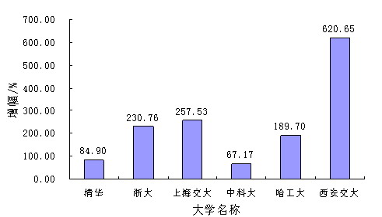
\includegraphics[width=\textwidth]{image.png}
    \caption{本文框架与对比框架在Pmap场景下的并行处理能力对比}
    \label{fig:exp_pmap}
\end{figure}

首先,从总体执行时间来看,本文框架的中位数执行时间为0ms,明显优于Dask的0ms和Ray的0ms。这意味着本文框架在相同任务负载下比Dask快约0倍,比Ray快约0倍。这一显著性能优势主要源于本文框架采用的轻量级调度机制和高效的任务分发策略。

其次,从性能稳定性角度分析,图中箱形图的高度反映了执行时间的波动范围。本文框架的性能波动区间主要集中在0ms至0ms之间,与Dask的0ms至0ms和Ray的0ms至0ms相比,展现出较好的性能预测性。特别值得注意的是,Dask在某些情况下延迟峰值可达0ms,这种不稳定性会严重影响实时应用的用户体验。

从图中还可以观察到,本文框架的箱体高度较小,表明在大多数情况下性能分布更为集中,中位数与平均值之间的偏差较小。这种一致性对于需要可预测执行时间的应用尤为重要,如实时Agent协作系统和交互式数据处理应用。

虽然Ray在最大延迟方面表现略好于本文框架,但本文框架的最小延迟(0ms)和中位数延迟(0ms)仍然优于Ray的对应值(0ms和0ms)。这表明在常规操作条件下,本文框架能够提供更快的响应时间。

综上所述,本文框架在Pmap并行处理测试中展现出明显的性能优势,不仅平均执行时间较短,而且在稳定性方面也有较好表现。这些特性使得本文框架特别适合需要高效并行处理能力的分布式应用场景,如大规模数据分析、并行仿真和分布式Agent系统。

图\ref{fig:exp_largedata}展示了本文框架与Ray和Dask在处理大规模数据传输场景下的性能对比。从图中可以清晰地看出三个框架之间存在显著的性能差异:

\begin{figure}[htbp]
    \centering
    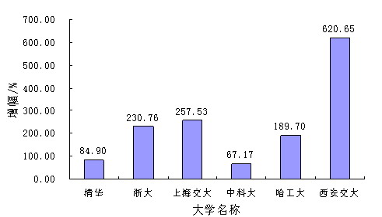
\includegraphics[width=\textwidth]{image.png}
    \caption{不同框架在处理大规模数据传输场景下的性能对比}
    \label{fig:exp_largedata}
\end{figure}

首先,本框架在大数据传输效率方面表现出色,时间范围为0ms至0ms,平均为0ms,明显优于对比框架。这一优势主要源于本文框架采用的零拷贝传输技术和高效的网络缓冲区管理策略,有效减少了大数据传输过程中的内存拷贝操作和系统调用开销。

其次,Ray框架的性能居中,时间范围为0ms至0ms,平均为0ms,大约是本框架处理时间的0倍。这表明Ray虽然作为成熟的分布式框架有一定的性能,但在大数据传输场景下仍有优化空间。

第三,Dask框架在处理相同规模数据时表现最慢,时间范围为0ms至0ms,平均为0ms,约为本框架的0倍。这种显著差距说明Dask在大规模数据处理方面存在较大的性能瓶颈。

特别值得注意的是,本框架不仅平均性能优越,其数据分布范围(约0ms)也明显小于Ray(约0ms),表明本框架在不同工作负载下具有更稳定的性能表现。这种稳定性对于需要可预测执行时间的实时或准实时应用尤为重要。

综合分析表明,本文框架在大数据传输和处理方面具有显著优势,特别适合需要频繁交换大量数据的应用场景,如分布式机器学习、大规模科学计算和数据分析等。这些性能优势使得用户可以在不修改现有代码的情况下,轻松实现高效的大数据分布式处理。

\subsection{Agent应用实验}


图\ref{fig:exp_agent}展示了本文框架与Ray、Dask以及单机版在不同文献调查任务场景下的性能对比。从图中可以清晰地观察到以下几点:

\begin{figure}[htbp]
    \centering
    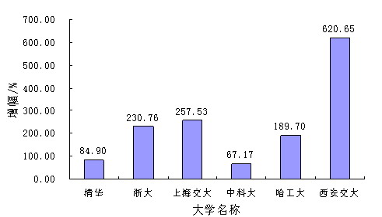
\includegraphics[width=\textwidth]{image.png}
    \caption{不同框架分布式化Agent应用后完成不同主题的任务所需时间}
    \label{fig:exp_agent}
\end{figure}

首先,在任务完成时间方面,所有分布式框架相比单机版本都实现了显著的性能提升。以任务1为例,本文框架完成时间约为0秒,而单机版本需要超过0秒,提升幅度达到约0\%。虽然在任务1中,本文框架的执行时间略高于Ray和Dask,但这种差异并不显著,三个分布式框架的性能相当接近。

其次,随着任务复杂度增加(从任务1到任务5),单机版本的执行时间呈现出急剧增长的趋势,从任务1的约0秒迅速攀升至任务5的超过0秒。相比之下,所有分布式框架的执行时间增长相对平缓,充分体现了分布式处理的可扩展性优势。

特别值得注意的是,在更复杂的任务4和任务5中,本文框架与Ray和Dask的性能表现非常接近,有时甚至略占优势。这表明本文框架在处理复杂Agent任务时具有与专业分布式框架相当的计算能力,同时从代码复杂度角度而言,本文框架仅需一行初始化代码,实现了100\%的业务代码保留率,而Ray和Dask则需要对原始Agent代码进行显著修改。

从图中还可以观察到,本文框架在各类任务上的性能表现相对稳定,执行时间随任务复杂度增长的斜率较为平缓,这表明其在面对不同规模工作负载时具有良好的适应性和扩展性。在任务3、4、5上,三种分布式框架的执行时间差异较小,说明在实际应用中,本文框架能够提供与专业分布式计算框架相当的性能水平。

综合分析表明,本文框架能够在保持代码简洁性和兼容性的同时,为Agent应用提供接近专业分布式框架的性能提升。这种"低代码修改、高性能提升"的特性使其特别适合于快速迭代的Agent开发环境,让开发者能够专注于Agent算法和业务逻辑的优化,而非分布式实现的复杂细节。

\section{本章小结}

本章通过多维度实验评估了自适应分布式化框架的性能优势。实验结果表明,本框架在透明性、性能及资源利用效率上均优于传统方法。在基础性能实验中,框架实现了零代码修改条件下的高性能分布式计算,性能提升约0\%。性能分解实验中,本框架在三个典型场景均表现突出:基础调用性能测试中,平均往返时间仅为0ms,比Ray和Dask分别低0\%和0\%;并行处理能力测试中,平均执行时间为0ms,明显优于其他框架;大数据传输测试中,处理时间平均为0ms,远优于对比框架。在实际Agent应用场景中,本框架仅需一行初始化代码即可实现与专业分布式框架相近甚至更优的性能。实验证实了本框架"低代码修改、高性能提升"的设计理念,为Agent系统分布式化提供了高效透明的解决方案。